% !TeX root = kovetelmeny.tex
\newcommand{\pontMeret}{0.33}
\newcommand{\nagyOsztas}{0.7}
\newcommand{\kisOsztas}{0.33}
\newcommand{\jegyMagassag}{0.7}
\newcommand{\foTengelyTavolsag}{1}
\newcommand{\tengelyEltolas}{1.5}

\newcommand{\pontMarker}[5] %x0,y0,h,color,pont
{\draw[#4] (#1,#2)--++(0,#3) node[anchor=south]{#5} ++(0,-0.3)--++(0.6,0)--++(-0.1,-0.1)++(0.1,0.1)--++(-0.1,0.1);}
\newcommand{\jegyMarker}[6] %x0,y0,h,color,pont,jegy
{\draw[#4] (#1,#2)--++(0,#3) node[anchor=south]{#5} ++(0,-0.3)--++(0.6,0)--++(-0.1,-0.1)++(0.1,0.1)--++(-0.1,0.1) node[anchor=south,draw,yshift=0.5mm]{#6};}

\definecolor{darkgreen}{rgb}{0,0.7,0}
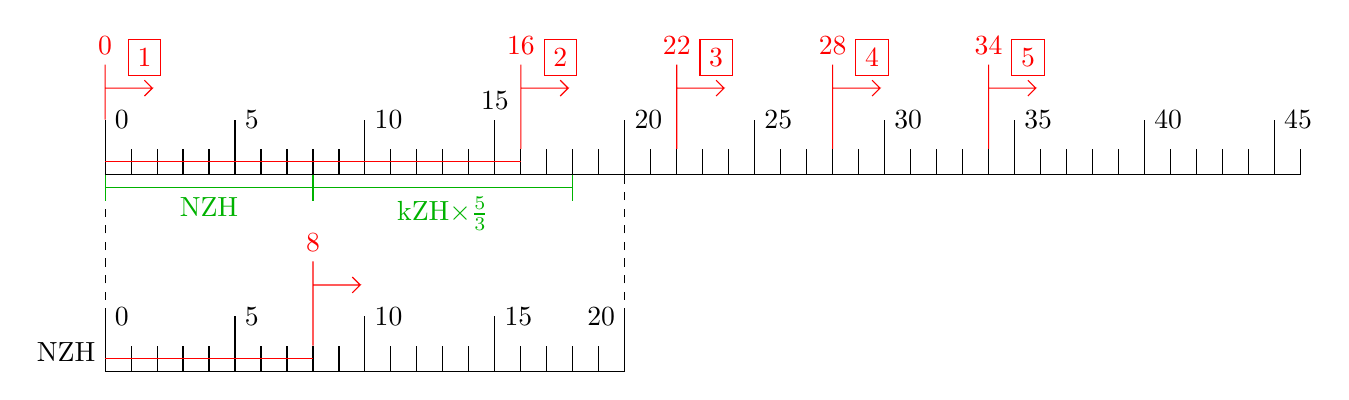
\begin{tikzpicture}
	% fő pontszám tengely és osztásai
	\draw (0,0)--(46*\pontMeret,0)
	(0,0)--++(0,\nagyOsztas) node[anchor=west]{$0$}
	(\pontMeret,0)--++(0,\kisOsztas)
	(2*\pontMeret,0)--++(0,\kisOsztas)
	(3*\pontMeret,0)--++(0,\kisOsztas)
	(4*\pontMeret,0)--++(0,\kisOsztas)
	(5*\pontMeret,0)--++(0,\nagyOsztas) node[anchor=west]{$5$}
	(6*\pontMeret,0)--++(0,\kisOsztas)
	(7*\pontMeret,0)--++(0,\kisOsztas)
	(8*\pontMeret,0)--++(0,\kisOsztas)
	(9*\pontMeret,0)--++(0,\kisOsztas)
	(10*\pontMeret,0)--++(0,\nagyOsztas) node[anchor=west]{$10$}
	(11*\pontMeret,0)--++(0,\kisOsztas)
	(12*\pontMeret,0)--++(0,\kisOsztas)
	(13*\pontMeret,0)--++(0,\kisOsztas)
	(14*\pontMeret,0)--++(0,\kisOsztas)
	(15*\pontMeret,0)--++(0,\nagyOsztas) node[anchor=south]{$15$}
	(16*\pontMeret,0)--++(0,\kisOsztas)
	(17*\pontMeret,0)--++(0,\kisOsztas)
	(18*\pontMeret,0)--++(0,\kisOsztas)
	(19*\pontMeret,0)--++(0,\kisOsztas)
	(20*\pontMeret,0)--++(0,\nagyOsztas) node[anchor=west]{$20$}
	(21*\pontMeret,0)--++(0,\kisOsztas)
	(22*\pontMeret,0)--++(0,\kisOsztas)
	(23*\pontMeret,0)--++(0,\kisOsztas)
	(24*\pontMeret,0)--++(0,\kisOsztas)
	(25*\pontMeret,0)--++(0,\nagyOsztas) node[anchor=west]{$25$}
	(26*\pontMeret,0)--++(0,\kisOsztas)
	(27*\pontMeret,0)--++(0,\kisOsztas)
	(28*\pontMeret,0)--++(0,\kisOsztas)
	(29*\pontMeret,0)--++(0,\kisOsztas)
	(30*\pontMeret,0)--++(0,\nagyOsztas) node[anchor=west]{$30$}
	(31*\pontMeret,0)--++(0,\kisOsztas)
	(32*\pontMeret,0)--++(0,\kisOsztas)
	(33*\pontMeret,0)--++(0,\kisOsztas)
	(34*\pontMeret,0)--++(0,\kisOsztas)
	(35*\pontMeret,0)--++(0,\nagyOsztas) node[anchor=west]{$35$}
	(36*\pontMeret,0)--++(0,\kisOsztas)
	(37*\pontMeret,0)--++(0,\kisOsztas)
	(38*\pontMeret,0)--++(0,\kisOsztas)
	(39*\pontMeret,0)--++(0,\kisOsztas)
	(40*\pontMeret,0)--++(0,\nagyOsztas) node[anchor=west]{$40$}
	(41*\pontMeret,0)--++(0,\kisOsztas)
	(42*\pontMeret,0)--++(0,\kisOsztas)
	(43*\pontMeret,0)--++(0,\kisOsztas)
	(44*\pontMeret,0)--++(0,\kisOsztas)
	(45*\pontMeret,0)--++(0,\nagyOsztas) node[anchor=west]{$45$}
	(46*\pontMeret,0)--++(0,\kisOsztas);
	% féléves jegy ponthatárok
	\jegyMarker{0}{\nagyOsztas}{\jegyMagassag}{red}{$0$}{$1$}
	\jegyMarker{16*\pontMeret}{\kisOsztas}{\nagyOsztas-\kisOsztas+\jegyMagassag}{red}{$16$}{$2$}
	\jegyMarker{22*\pontMeret}{\kisOsztas}{\nagyOsztas-\kisOsztas+\jegyMagassag}{red}{$22$}{$3$}
	\jegyMarker{28*\pontMeret}{\kisOsztas}{\nagyOsztas-\kisOsztas+\jegyMagassag}{red}{$28$}{$4$}
	\jegyMarker{34*\pontMeret}{\kisOsztas}{\nagyOsztas-\kisOsztas+\jegyMagassag}{red}{$34$}{$5$}
	\draw[red] (0,0.5*\kisOsztas)--++(16*\pontMeret,0);
	% NHZ tengely
	\draw (0,-\foTengelyTavolsag-\tengelyEltolas) node[anchor=south east]{NZH} --++(20*\pontMeret,0)
	(0,-\foTengelyTavolsag-\tengelyEltolas)--++(0,\nagyOsztas) node[anchor=west]{$0$}
	(\pontMeret,-\foTengelyTavolsag-\tengelyEltolas)--++(0,\kisOsztas)
	(2*\pontMeret,-\foTengelyTavolsag-\tengelyEltolas)--++(0,\kisOsztas)
	(3*\pontMeret,-\foTengelyTavolsag-\tengelyEltolas)--++(0,\kisOsztas)
	(4*\pontMeret,-\foTengelyTavolsag-\tengelyEltolas)--++(0,\kisOsztas)
	(5*\pontMeret,-\foTengelyTavolsag-\tengelyEltolas)--++(0,\nagyOsztas) node[anchor=west]{$5$}
	(6*\pontMeret,-\foTengelyTavolsag-\tengelyEltolas)--++(0,\kisOsztas)
	(7*\pontMeret,-\foTengelyTavolsag-\tengelyEltolas)--++(0,\kisOsztas)
	(8*\pontMeret,-\foTengelyTavolsag-\tengelyEltolas)--++(0,\kisOsztas)
	(9*\pontMeret,-\foTengelyTavolsag-\tengelyEltolas)--++(0,\kisOsztas)
	(10*\pontMeret,-\foTengelyTavolsag-\tengelyEltolas)--++(0,\nagyOsztas) node[anchor=west]{$10$}
	(11*\pontMeret,-\foTengelyTavolsag-\tengelyEltolas)--++(0,\kisOsztas)
	(12*\pontMeret,-\foTengelyTavolsag-\tengelyEltolas)--++(0,\kisOsztas)
	(13*\pontMeret,-\foTengelyTavolsag-\tengelyEltolas)--++(0,\kisOsztas)
	(14*\pontMeret,-\foTengelyTavolsag-\tengelyEltolas)--++(0,\kisOsztas)
	(15*\pontMeret,-\foTengelyTavolsag-\tengelyEltolas)--++(0,\nagyOsztas) node[anchor=west]{$15$}
	(16*\pontMeret,-\foTengelyTavolsag-\tengelyEltolas)--++(0,\kisOsztas)
	(17*\pontMeret,-\foTengelyTavolsag-\tengelyEltolas)--++(0,\kisOsztas)
	(18*\pontMeret,-\foTengelyTavolsag-\tengelyEltolas)--++(0,\kisOsztas)
	(19*\pontMeret,-\foTengelyTavolsag-\tengelyEltolas)--++(0,\kisOsztas)
	(20*\pontMeret,-\foTengelyTavolsag-\tengelyEltolas)--++(0,\nagyOsztas) node[anchor=east]{$20$};
	\draw [dashed] (0,-\foTengelyTavolsag-\tengelyEltolas+\nagyOsztas)--(0,0)
	(20*\pontMeret,-\foTengelyTavolsag-\tengelyEltolas+\nagyOsztas)--(20*\pontMeret,0);
	% NZH követelmény
	\pontMarker{8*\pontMeret}{-\foTengelyTavolsag-\tengelyEltolas+\kisOsztas}{\nagyOsztas-\kisOsztas+\jegyMagassag}{red}{$8$}
	\draw[red] (0,-\foTengelyTavolsag-\tengelyEltolas+0.5*\kisOsztas)--++(8*\pontMeret,0);
	% 16 minimumpont teljesítése
	\draw[darkgreen] (0,-0.5*\kisOsztas)--++(18*\pontMeret,0)
	(0,0)--++(0,-\kisOsztas)
	(8*\pontMeret,0)--++(0,-\kisOsztas)
	(18*\pontMeret,0)--++(0,-\kisOsztas);
	\node at(4*\pontMeret,-0.5*\kisOsztas)[anchor=north,darkgreen]{NZH};
	\node at(13*\pontMeret,-0.5*\kisOsztas)[anchor=north,darkgreen]{kZH$\times\frac{5}{3}$};
\end{tikzpicture}